A heuristic is a practical problem-solving technique designed to produce good-enough solutions within a reasonable time frame, 
especially when exact methods are too slow or infeasible. Given the NP-hard nature of the Travelling Salesman Problem (TSP), 
computing the optimal solution can be computationally expensive even for moderately sized instances. For this reason, heuristic methods 
play a crucial role in tackling the problem efficiently. Heuristics do not guarantee optimality, but they can often yield solutions 
that are sufficiently close to the best possible one. This trade-off between accuracy and speed makes heuristics particularly valuable 
when timely decision-making is more important than absolute precision.

In this chapter, several heuristic strategies for the TSP are presented, highlighting their underlying principles, implementation, and performance.

\section{Nearest Neighbour - Greedy}

One of the most intuitive heuristic approaches to the Travelling Salesman Problem is the \textbf{Nearest Neighbor} (NN) algorithm, which follows a greedy strategy. 
A \textit{greedy} algorithm builds a solution step by step by always choosing the locally optimal option, with the hope that this leads to a good global solution.
In the context of the TSP, the algorithm starts from an initial node and, at each iteration, selects the nearest unvisited node as the next step in the tour. 
This process continues until all nodes have been visited exactly once, and the cycle is closed by returning to the starting point.
However, the quality of the solution obtained using this method depends heavily on the starting node, as different starting points may lead to significantly 
different tours.
While NN is fast and easy to implement, its performance depends heavily on the starting node and often produces suboptimal solutions. Still, it often produces a reasonable approximation in a fraction of the time required by exact methods, making it suitable for large instances where exact algorithms are computationally expensive.

\begin{algorithm}
\caption{Nearest Neighbor Heuristic}
\begin{algorithmic}
  \Require Starting node $s \in V$
  \Ensure Hamiltonian cycle of $G$, cost of cycle
  \State $cycle \gets [s]$
  \State $cost \gets 0$
  \For{$i \gets 0$ to $|V| - 2$}
    \State $next \gets \arg\min_{v \in V \setminus cycle} c(cycle[i], v)$
    \State $cost \gets cost + c(cycle[i], next)$
    \State $cycle[i+1] \gets next$
  \EndFor
  \State $cost \gets cost + c(cycle[|V| - 1], s)$
  \State \Return $cycle$, $cost$
\end{algorithmic}
\end{algorithm}

\subsection{Results Analysis}
\label{sec:nn-analysis}
The greedy algorithm often selects locally optimal edges without considering long-term implications, which may lead to expensive connections, 
especially when few unvisited nodes remain. This behavior can result in unnecessarily long edges and poor-quality tours. Such issues are particularly 
evident in Euclidean instances, where the resulting path may include edge crossings, which are absent in optimal solutions.

\begin{figure}[h!]
    \centering
    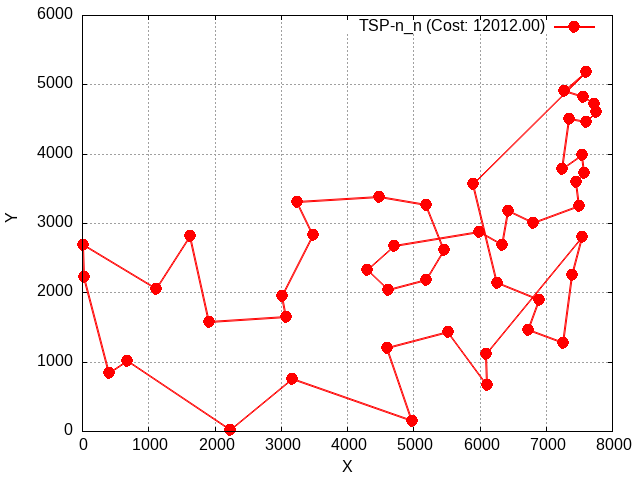
\includegraphics[width=0.7\textwidth]{images/TSP_n_n.png}
    \caption{Nearest Neighbor heuristic solution.}
    \label{fig:nn-example}
\end{figure}

Figure~\ref{fig:nn-example} illustrates the best tour obtained by running the Nearest Neighbor heuristic from each possible starting node on the \textit{Att48} instance. Several edge crossings are visible, indicating inefficiencies. The resulting tour cost is \textbf{12012}, significantly higher than the optimal cost of \textbf{10628}.

To address these limitations, the next section introduces the 2-opt heuristic, a simple yet effective local search technique aimed at improving tour quality by eliminating such inefficiencies.

\section{Two-Opt}

The \textit{2-opt} algorithm is a local search optimization technique designed to improve a given (possibly sub-optimal) tour 
in the Travelling Salesman Problem. It works by iteratively removing two edges from the tour and reconnecting the resulting paths 
in the opposite way, with the goal of reducing the overall cost of the cycle.
Formally, we can interpret 2-opt as a particular case of a more general class of heuristics known as \textit{k-opt}, 
where $k$ edges are removed and reconnected to form a new valid tour. In the 2-opt case, we identify two edges $(p_i, p_{i+1})$ 
and $(p_j, p_{j+1})$ such that replacing them with $(p_i, p_j)$ and $(p_{i+1}, p_{j+1})$, while reversing the intermediate segment between $p_{i+1}$ and $p_j$. 
The necessary condition for this move to be beneficial is:

The 2-opt move is beneficial only if replacing the two selected edges reduces the overall tour cost. 
Consider the current edges \((p_i, p_{i+1})\) and \((p_j, p_{j+1})\). 
We propose replacing them with \((p_i, p_j)\) and \((p_{i+1}, p_{j+1})\), 
which effectively reverses the intermediate segment of the tour.

The move is accepted if the total cost decreases, i.e., if:

\begin{equation}
    c(p_i, p_{i+1}) + c(p_j, p_{j+1}) > c(p_i, p_j) + c(p_{i+1}, p_{j+1})
    \label{eq:2opt-condition}
\end{equation}

Equivalently, the cost change \(\Delta\) resulting from this move can be computed as:

\begin{equation}
    \Delta = [c(p_i, p_j) + c(p_{i+1}, p_{j+1})] - [c(p_i, p_{i+1}) + c(p_j, p_{j+1})]
    \label{eq:2opt-delta}
\end{equation}

If \(\Delta < 0\), the move yields a shorter tour and is therefore accepted.

After identifying such a pair of edges, the segment of the tour between nodes $p_{i+1}$ and $p_j$ is reversed to maintain tour feasibility.

\begin{figure}[H]
    \centering
    \begin{subfigure}[c]{.4\textwidth}
        \centering
        \begin{tikzpicture}
            \begin{scope}[every node/.style={circle,thick,draw}]
                \node (I) at (0,0) {$p_i$};
                \node (JJ) at (0,3) {$p_{j+1}$};
                \node (II) at (2.5,4) {$p_{i+1}$};
                \node (J) at (4.5,1) {$p_j$};
            \end{scope}
            \begin{scope}[>={Stealth[black]}, every node/.style={fill=white,circle},
                          every edge/.style={draw=red,very thick}]
                \draw[->,black] (I) -- (II);
                \draw[->,black] (J) -- (JJ);
            \end{scope}
        \end{tikzpicture}
        \caption{Before the move}
    \end{subfigure}
    \hfill
    \begin{subfigure}[c]{.4\textwidth}
        \centering
        \begin{tikzpicture}
            \begin{scope}[every node/.style={circle,thick,draw}]
                \node (I) at (0,0) {$p_i$};
                \node (JJ) at (0,3) {$p_{j+1}$};
                \node (II) at (2.5,4) {$p_{i+1}$};
                \node (J) at (4.5,1) {$p_j$};
            \end{scope}
            \begin{scope}[>={Stealth[black]}, every node/.style={fill=white,circle},
                          every edge/.style={draw=blue,very thick}]
                \draw[->,blue] (I) -- (J);
                \draw[->,blue] (II) -- (JJ);
            \end{scope}
        \end{tikzpicture}
        \caption{After the move}
    \end{subfigure}
    \caption{Example of a 2-opt move eliminating edge crossing.}
    \label{fig:2optmove}
\end{figure}


As shown in Figure~\ref{fig:2optmove}, this operation is particularly useful in Euclidean instances, where removing intersecting edges 
usually improves the tour cost significantly. The process is repeated iteratively: at each step, the algorithm scans the tour looking 
for a pair of edges satisfying the inequality. If found, the edges are swapped and the search continues. 
When no further improvement can be found, the procedure terminates. This yields a solution that is often significantly better than the initial one, 
although not necessarily optimal.

To improve the Nearest Neighbor result, the 2-opt heuristic is applied as a post-processing step to the best tour found among all possible NN starting nodes. This selective refinement avoids unnecessary computation while still producing a significantly improved solution.

\subsection{Pseudocode}

\begin{algorithm}
\caption{Two-Opt Heuristic for TSP}
\label{alg:twoopt}
\textbf{Input:} A Hamiltonian cycle \texttt{solution} of a graph $G$, with associated cost\\
\textbf{Output:} An improved Hamiltonian cycle (locally optimal w.r.t. 2-opt), updated cost
\begin{algorithmic}
\Procedure{ApplyTwoOpt}{$solution$, $nnodes$}
    \State $improved \gets$ \textbf{true}
    \While{$improved$}
        \State $improved \gets$ \textbf{false}
        \For{$i \gets 0$ \textbf{to} $nnodes - 2$}
            \For{$j \gets i + 1$ \textbf{to} $nnodes - 1$}
                \State $\Delta \gets$ \Call{CostDelta}{$i$, $j$, $solution$}
                \If{$\Delta < 0$}
                    \State \Call{ReverseSubsequence}{$solution$, $i + 1$, $j$}
                    \State $solution.cost \gets solution.cost + \Delta$
                    \State $improved \gets$ \textbf{true}
                \EndIf
            \EndFor
        \EndFor
    \EndWhile
    \State \Return $solution$
\EndProcedure
\end{algorithmic}
\end{algorithm}

\begin{algorithm}
\caption{CostDelta and Subsequence Reversal}
\label{alg:subroutines}
\begin{algorithmic}
\Function{CostDelta}{$i$, $j$, $solution$}
    \State Let $p_i, p_{i+1}, p_j, p_{j+1}$ be the involved nodes
    \State \Return $c(p_i, p_j) + c(p_{i+1}, p_{j+1}) - c(p_i, p_{i+1}) - c(p_j, p_{j+1})$
\EndFunction

\Procedure{ReverseSubsequence}{$solution$, $start$, $end$}
    \State Reverse the order of nodes in $solution$ between indices $start$ and $end$ (inclusive)
\EndProcedure
\end{algorithmic}
\end{algorithm}

The \texttt{ApplyTwoOpt} procedure iteratively applies improving 2-opt moves until no further improvement is possible. 
The cost difference \texttt{CostDelta} evaluates the gain of removing two edges and reconnecting them in the opposite direction. 
If an improvement is found, the affected segment of the tour is reversed.

\subsection{Results Analysis}
To prove the effectiveness of the 2-opt approach, we apply it to the best tour generated by NN heuristic presented in Section \ref{sec:nn-analysis}.
Figure \ref{fig:nn-2opt-example} shows how this technique is as simple as it is effective. All edge crossings have been eliminated, resulting in a visibly more efficient tour.

\begin{figure}[h!]
    \centering
    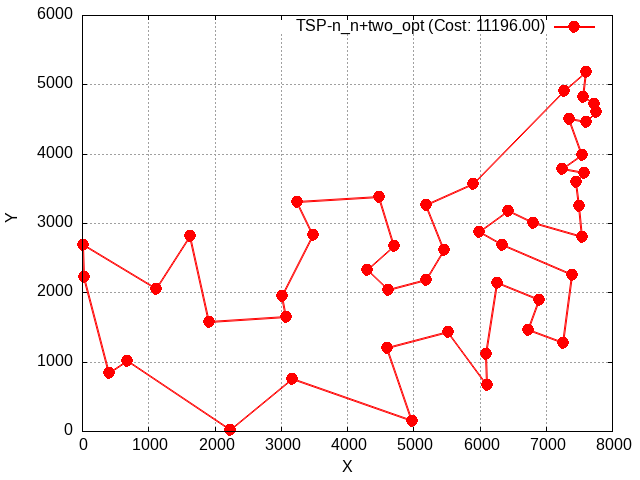
\includegraphics[width=0.7\textwidth]{images/TSP_n_n+two_opt.png}
    \caption{2-opt solution applied to the best tour generated by NN.}
    \label{fig:nn-2opt-example}
\end{figure}

To evaluate the improvement quantitatively, we can compare the cost of the tour before and after applying 2-opt and the computing time required to run both approaches. Table \ref{tab:nn-vs-2opt} summarizes the results of this comparison and highlights the significant reduction in tour cost achieved by the 2-opt heuristic, as well as the minimal increase in computation time.

\begin{table}[h!]
    \centering
    \caption{Comparison of tour cost and computation time.}
    \begin{tabular}{|c|c|c|}
        \hline
        Strategy & Cost & Time \\
        \hline
        NN        & 12012 & 0.006172 s \\
        \textbf{NN + 2opt} & \textbf{11196} & \textbf{0.006461 s} \\
        \hline
    \end{tabular}
    \label{tab:nn-vs-2opt}
\end{table}

These results are only meant to give an idea of the effectiveness of the 2-opt heuristic, some more rigorous analysis will be presented in Section XX \todo[inline]{Aggiungere riferimento alla sezione analisi perfprof}
